% Options for packages loaded elsewhere
\PassOptionsToPackage{unicode}{hyperref}
\PassOptionsToPackage{hyphens}{url}
%
\documentclass[
]{book}
\usepackage{lmodern}
\usepackage{amssymb,amsmath}
\usepackage{ifxetex,ifluatex}
\ifnum 0\ifxetex 1\fi\ifluatex 1\fi=0 % if pdftex
  \usepackage[T1]{fontenc}
  \usepackage[utf8]{inputenc}
  \usepackage{textcomp} % provide euro and other symbols
\else % if luatex or xetex
  \usepackage{unicode-math}
  \defaultfontfeatures{Scale=MatchLowercase}
  \defaultfontfeatures[\rmfamily]{Ligatures=TeX,Scale=1}
\fi
% Use upquote if available, for straight quotes in verbatim environments
\IfFileExists{upquote.sty}{\usepackage{upquote}}{}
\IfFileExists{microtype.sty}{% use microtype if available
  \usepackage[]{microtype}
  \UseMicrotypeSet[protrusion]{basicmath} % disable protrusion for tt fonts
}{}
\makeatletter
\@ifundefined{KOMAClassName}{% if non-KOMA class
  \IfFileExists{parskip.sty}{%
    \usepackage{parskip}
  }{% else
    \setlength{\parindent}{0pt}
    \setlength{\parskip}{6pt plus 2pt minus 1pt}}
}{% if KOMA class
  \KOMAoptions{parskip=half}}
\makeatother
\usepackage{xcolor}
\IfFileExists{xurl.sty}{\usepackage{xurl}}{} % add URL line breaks if available
\IfFileExists{bookmark.sty}{\usepackage{bookmark}}{\usepackage{hyperref}}
\hypersetup{
  pdftitle={Bayesian Inference with Bayes Factors},
  pdfauthor={Dan MacLean},
  hidelinks,
  pdfcreator={LaTeX via pandoc}}
\urlstyle{same} % disable monospaced font for URLs
\usepackage{color}
\usepackage{fancyvrb}
\newcommand{\VerbBar}{|}
\newcommand{\VERB}{\Verb[commandchars=\\\{\}]}
\DefineVerbatimEnvironment{Highlighting}{Verbatim}{commandchars=\\\{\}}
% Add ',fontsize=\small' for more characters per line
\usepackage{framed}
\definecolor{shadecolor}{RGB}{248,248,248}
\newenvironment{Shaded}{\begin{snugshade}}{\end{snugshade}}
\newcommand{\AlertTok}[1]{\textcolor[rgb]{0.94,0.16,0.16}{#1}}
\newcommand{\AnnotationTok}[1]{\textcolor[rgb]{0.56,0.35,0.01}{\textbf{\textit{#1}}}}
\newcommand{\AttributeTok}[1]{\textcolor[rgb]{0.77,0.63,0.00}{#1}}
\newcommand{\BaseNTok}[1]{\textcolor[rgb]{0.00,0.00,0.81}{#1}}
\newcommand{\BuiltInTok}[1]{#1}
\newcommand{\CharTok}[1]{\textcolor[rgb]{0.31,0.60,0.02}{#1}}
\newcommand{\CommentTok}[1]{\textcolor[rgb]{0.56,0.35,0.01}{\textit{#1}}}
\newcommand{\CommentVarTok}[1]{\textcolor[rgb]{0.56,0.35,0.01}{\textbf{\textit{#1}}}}
\newcommand{\ConstantTok}[1]{\textcolor[rgb]{0.00,0.00,0.00}{#1}}
\newcommand{\ControlFlowTok}[1]{\textcolor[rgb]{0.13,0.29,0.53}{\textbf{#1}}}
\newcommand{\DataTypeTok}[1]{\textcolor[rgb]{0.13,0.29,0.53}{#1}}
\newcommand{\DecValTok}[1]{\textcolor[rgb]{0.00,0.00,0.81}{#1}}
\newcommand{\DocumentationTok}[1]{\textcolor[rgb]{0.56,0.35,0.01}{\textbf{\textit{#1}}}}
\newcommand{\ErrorTok}[1]{\textcolor[rgb]{0.64,0.00,0.00}{\textbf{#1}}}
\newcommand{\ExtensionTok}[1]{#1}
\newcommand{\FloatTok}[1]{\textcolor[rgb]{0.00,0.00,0.81}{#1}}
\newcommand{\FunctionTok}[1]{\textcolor[rgb]{0.00,0.00,0.00}{#1}}
\newcommand{\ImportTok}[1]{#1}
\newcommand{\InformationTok}[1]{\textcolor[rgb]{0.56,0.35,0.01}{\textbf{\textit{#1}}}}
\newcommand{\KeywordTok}[1]{\textcolor[rgb]{0.13,0.29,0.53}{\textbf{#1}}}
\newcommand{\NormalTok}[1]{#1}
\newcommand{\OperatorTok}[1]{\textcolor[rgb]{0.81,0.36,0.00}{\textbf{#1}}}
\newcommand{\OtherTok}[1]{\textcolor[rgb]{0.56,0.35,0.01}{#1}}
\newcommand{\PreprocessorTok}[1]{\textcolor[rgb]{0.56,0.35,0.01}{\textit{#1}}}
\newcommand{\RegionMarkerTok}[1]{#1}
\newcommand{\SpecialCharTok}[1]{\textcolor[rgb]{0.00,0.00,0.00}{#1}}
\newcommand{\SpecialStringTok}[1]{\textcolor[rgb]{0.31,0.60,0.02}{#1}}
\newcommand{\StringTok}[1]{\textcolor[rgb]{0.31,0.60,0.02}{#1}}
\newcommand{\VariableTok}[1]{\textcolor[rgb]{0.00,0.00,0.00}{#1}}
\newcommand{\VerbatimStringTok}[1]{\textcolor[rgb]{0.31,0.60,0.02}{#1}}
\newcommand{\WarningTok}[1]{\textcolor[rgb]{0.56,0.35,0.01}{\textbf{\textit{#1}}}}
\usepackage{longtable,booktabs}
% Correct order of tables after \paragraph or \subparagraph
\usepackage{etoolbox}
\makeatletter
\patchcmd\longtable{\par}{\if@noskipsec\mbox{}\fi\par}{}{}
\makeatother
% Allow footnotes in longtable head/foot
\IfFileExists{footnotehyper.sty}{\usepackage{footnotehyper}}{\usepackage{footnote}}
\makesavenoteenv{longtable}
\usepackage{graphicx,grffile}
\makeatletter
\def\maxwidth{\ifdim\Gin@nat@width>\linewidth\linewidth\else\Gin@nat@width\fi}
\def\maxheight{\ifdim\Gin@nat@height>\textheight\textheight\else\Gin@nat@height\fi}
\makeatother
% Scale images if necessary, so that they will not overflow the page
% margins by default, and it is still possible to overwrite the defaults
% using explicit options in \includegraphics[width, height, ...]{}
\setkeys{Gin}{width=\maxwidth,height=\maxheight,keepaspectratio}
% Set default figure placement to htbp
\makeatletter
\def\fps@figure{htbp}
\makeatother
\setlength{\emergencystretch}{3em} % prevent overfull lines
\providecommand{\tightlist}{%
  \setlength{\itemsep}{0pt}\setlength{\parskip}{0pt}}
\setcounter{secnumdepth}{5}
\usepackage{booktabs}
\usepackage{tcolorbox}
\usepackage{quotchap}

\usepackage[T1]{fontenc}
\usepackage{amsthm}
\makeatletter
\def\thm@space@setup{%
  \thm@preskip=8pt plus 2pt minus 4pt
  \thm@postskip=\thm@preskip
}
\makeatother
\setmainfont[UprightFeatures={SmallCapsFont=AlegreyaSC-Regular}]{Alegreya}
\renewcommand{\textfraction}{0.05}
\renewcommand{\topfraction}{0.8}
\renewcommand{\bottomfraction}{0.8}
\renewcommand{\floatpagefraction}{0.75}
\let\oldhref\href
\renewcommand{\href}[2]{#2\footnote{\url{#1}}}

\newenvironment{task}
{ \begin{tcolorbox}[title=For you to do,title filled] }
{  \end{tcolorbox} }

\newenvironment{reader}
{ \begin{tcolorbox}[colbacktitle=red!50!white,
title=huh?,coltitle=white,
fonttitle=\bfseries] }
{  \end{tcolorbox} }

% \newenvironment{roundup}
% { \begin{tcolorbox}[colbacktitle=yellow!50!white,title=Round Up,title filled] }
%{  \end{tcolorbox} }

\newenvironment{myquote}
{\begin{large}
\begin{itshape}
\begin{minipage}{6cm}
}
{
\begin{vspace}{15mm}
\end{vspace}
\end{minipage}
\end{itshape}
\end{large}
}

\newenvironment{sidenote}
{ \begin{tcolorbox}[colbacktitle=blue!50!white,
title=huh?,coltitle=white,
fonttitle=\bfseries] }
{  \end{tcolorbox} }

\newenvironment{roundup}
{ \begin{tcolorbox}[colbacktitle=yellow!50!white,
title=Round Up,coltitle=black,
fonttitle=\bfseries] }
{  \end{tcolorbox} }
\usepackage[]{natbib}
\bibliographystyle{apalike}

\title{Bayesian Inference with Bayes Factors}
\author{Dan MacLean}
\date{2021-02-26}

\begin{document}
\maketitle

{
\setcounter{tocdepth}{1}
\tableofcontents
}
\hypertarget{setting-up}{%
\chapter{Setting up}\label{setting-up}}

The primary purpose of this course is to help you to understand how to use statistics that will help with your research. The course will try to explain a branch of statistics called `Estimation Statistics' which are complementary to the normal sort of hypothesis test procedures and address some of the criticisms of those methods.

Statistics is a computationally heavy topic, so we'll be making use of the R statistical programming environment to do that side of the work. The rest of this chapter will help you get that set up on your own computer.

\hypertarget{prerequisites}{%
\section{Prerequisites}\label{prerequisites}}

\hypertarget{knowledge-prerequisites}{%
\subsection{Knowledge prerequisites}\label{knowledge-prerequisites}}

There are no specific knowledge prerequisites for this book but it will be very helpful if you have read and worked through the \texttt{ggplot}, \texttt{Intro\ to\ Stats} and \texttt{Estimation\ Statistics} books and are familiar with R use.

\hypertarget{software-prerequisites}{%
\subsection{Software prerequisites}\label{software-prerequisites}}

You need to install the following stuff for this book:

\begin{enumerate}
\def\labelenumi{\arabic{enumi}.}
\tightlist
\item
  R
\item
  RStudio
\item
  Some R packages: \texttt{devtools}, \texttt{tidyverse} and \texttt{BayesFactor} and \texttt{simplebf}
\end{enumerate}

\hypertarget{installing-r}{%
\section{Installing R}\label{installing-r}}

Follow this link and install the right version for your operating system \url{https://www.stats.bris.ac.uk/R/}

\hypertarget{installing-rstudio}{%
\section{Installing RStudio}\label{installing-rstudio}}

Follow this link and install the right version for your operating system \url{https://www.rstudio.com/products/rstudio/download/}

\hypertarget{installing-r-packages-in-rstudio}{%
\section{Installing R packages in RStudio}\label{installing-r-packages-in-rstudio}}

\hypertarget{standard-packages}{%
\subsection{Standard packages}\label{standard-packages}}

In the RStudio console, type

\texttt{install.packages(c("tidyverse",\ "BayesFactor"))}

and these packages should install. Once that is done, type

\texttt{devtools::install\_github("danmaclean/simplebf")}

to install the final package

\hypertarget{motivation}{%
\chapter{Motivation}\label{motivation}}

The sort of statistics that most experimental science students are taught are called `Frequentist Statistics'. They include the \(t\)-tests, ANOVA and \(\chi^2\)-tests and the linear models that we have studied already.

The inferential approach in the Frequentist paradigm is often criticised for being weak and is often abused. Although the abuse is as much a consequence of convention in the scientific literature and in scientific publishing, the misinterpretation of \(p\)-values by generations of scientists as it is the philosophical weakness of the methods themselves, the weaknesses persist and over time other paradigms have emerged.

We have seen an alternative in Estimation Statistics, in this book we will look at another - Bayesian Inference and using Bayes Factors to compare levels of evidence for one hypothesis over another, rather than just accepting or rejecting a simplistic null hypothesis.

The advantage of this will be that we can much more directly select between specific hypotheses that might describe our data. This will give us a much clearer idea about a question that we instinctively want to answer when we do statistics - `Which hypothesis is most likely true?', we will see that we can formulate this in lots of ways, but in general the hypotheses we want to compare will be something along the lines of some measured quantity being different in different samples. With Frequentist Inference we can only ask the roundabout question, `How often does the difference we observe occur by chance?' and if it isn't likely, say so. With Bayes Factors we will be able to compare directly competing hypotheses and reject the least likely absolutely.

\hypertarget{mr.-micawbers-rule-of-statistical-inference}{%
\section{Mr.~Micawber's rule of statistical inference}\label{mr.-micawbers-rule-of-statistical-inference}}

The ruinous role of the \(p\)-value in modern science can not be overstated. This one value is responsible for happiness and dispair in equal measure. Dicken's Mr.~Micawber had this to say about the role of money in life's happiness:

\begin{quote}
`Annual income 20 pounds, annual expenditure 19 {[}pounds{]} 19 shillings and six pence, result happiness. Annual income 20 pounds, annual expenditure 20 pounds ought and six, result misery.'
\end{quote}

In science a corollary exists:

\begin{quote}
`\(p\) below 0.05, result success, papers, grants, and tenure. \(p\) above 0.05 result failure, misery, ignominy, and rejection.'
\end{quote}

The truth is that \(p < 0.05\) is an entirely arbitrary cut-off and is not in itself a helpful or meaningful value. Various scientific communities, led by publishing requirements, have accepted this a gold standard of truth against sense and often against rigorousness. With Bayesian tests we will be able to completely do away with \(p\)-values and confidence intervals and in their place use a more evidence based approach to making inferences.

\hypertarget{r-fundamentals}{%
\chapter{R Fundamentals}\label{r-fundamentals}}

\hypertarget{about-this-chapter}{%
\section{About this chapter}\label{about-this-chapter}}

\begin{enumerate}
\def\labelenumi{\arabic{enumi}.}
\tightlist
\item
  Questions:
\end{enumerate}

\begin{itemize}
\tightlist
\item
  How do I use R?
\end{itemize}

\begin{enumerate}
\def\labelenumi{\arabic{enumi}.}
\setcounter{enumi}{1}
\tightlist
\item
  Objectives:
\end{enumerate}

\begin{itemize}
\tightlist
\item
  Become familiar with R syntax
\item
  Understand the concepts of objects and assignment
\item
  Get exposed to a few functions
\end{itemize}

\begin{enumerate}
\def\labelenumi{\arabic{enumi}.}
\setcounter{enumi}{2}
\tightlist
\item
  Keypoints:
\end{enumerate}

\begin{itemize}
\tightlist
\item
  R's capabilities are provided by functions
\item
  R users call functions and get results
\end{itemize}

\hypertarget{working-with-r}{%
\section{Working with R}\label{working-with-r}}

In this workshop we'll use R in the extremely useful RStudio software. For the most part we'll work interactively, meaning we'll type stuff straight into the R console in RStudio (Usually this is a window on the left or lower left) and get our results there too (usually in the console or in a window on the right).

Panels like the ones below mimic the interaction with R and first show the thing to type into R, and below the calculated result from R.

Let's look at how R works by using it for it's most basic job - as a calculator:

\begin{Shaded}
\begin{Highlighting}[]
 \DecValTok{3} \OperatorTok{+}\StringTok{ }\DecValTok{5}
\end{Highlighting}
\end{Shaded}

\begin{verbatim}
## [1] 8
\end{verbatim}

\begin{Shaded}
\begin{Highlighting}[]
 \DecValTok{12} \OperatorTok{*}\StringTok{ }\DecValTok{2}
\end{Highlighting}
\end{Shaded}

\begin{verbatim}
## [1] 24
\end{verbatim}

\begin{Shaded}
\begin{Highlighting}[]
 \DecValTok{1} \OperatorTok{/}\StringTok{ }\DecValTok{3}
\end{Highlighting}
\end{Shaded}

\begin{verbatim}
## [1] 0.3333333
\end{verbatim}

\begin{Shaded}
\begin{Highlighting}[]
 \DecValTok{12} \OperatorTok{*}\StringTok{ }\DecValTok{2}
\end{Highlighting}
\end{Shaded}

\begin{verbatim}
## [1] 24
\end{verbatim}

Fairly straightforward, we type in the expression and we get a result. That's how this whole book will work, you type the stuff in, and get answers out. It'll be easiest to learn if you go ahead and copy the examples one by one. Try to resist the urge to use copy and paste. Typing longhand really encourages you to look at what you're entering.

As far as the R output itself goes, it's really straightforward - its just the answer with a \texttt{{[}1{]}} stuck on the front. This \texttt{{[}1{]}} tells us how many items through the output we are. Often R will return long lists of numbers and it can be helpful to have this extra information.

\hypertarget{variables}{%
\section{Variables}\label{variables}}

We can save the output of operations for later use by giving it a name using the assignment symbol \texttt{\textless{}-}. Read this symbol as `gets', so \texttt{x\ \textless{}-\ 5} reads as `x gets 5'. These names are called variables, because the value they are associated with can change.

Let's give five a name, \texttt{x} then refer to the value 5 by it's name. We can then use the name in place of the value. In the jargon of computing we say we are assigning a value to a variable.

\begin{Shaded}
\begin{Highlighting}[]
\NormalTok{ x <-}\StringTok{ }\DecValTok{5}
\NormalTok{ x}
\end{Highlighting}
\end{Shaded}

\begin{verbatim}
## [1] 5
\end{verbatim}

\begin{Shaded}
\begin{Highlighting}[]
\NormalTok{ x }\OperatorTok{*}\StringTok{ }\DecValTok{2}
\end{Highlighting}
\end{Shaded}

\begin{verbatim}
## [1] 10
\end{verbatim}

\begin{Shaded}
\begin{Highlighting}[]
\NormalTok{y <-}\StringTok{ }\DecValTok{3}
\NormalTok{x }\OperatorTok{*}\StringTok{ }\NormalTok{y}
\end{Highlighting}
\end{Shaded}

\begin{verbatim}
## [1] 15
\end{verbatim}

This is of course of limited value with just numbers but is of great value when we have large datasets, as the whole thing can be referred to by the variable.

\hypertarget{using-objects-and-functions}{%
\subsection{Using objects and functions}\label{using-objects-and-functions}}

At the top level, R is a simple language with two types of thing: functions and objects. As a user you will use functions to do stuff, and get back objects as an answer. Functions are easy to spot, they are a name followed by a pair of brackets. A function like \texttt{mean()} is the function for calculating a mean. The options (or arguments) for the function go inside the brackets:

\begin{Shaded}
\begin{Highlighting}[]
\KeywordTok{sqrt}\NormalTok{(}\DecValTok{16}\NormalTok{)}
\end{Highlighting}
\end{Shaded}

\begin{verbatim}
## [1] 4
\end{verbatim}

Often the result from a function will be more complicated than a simple number object, often it will be a vector (simple list), like from the \texttt{rnorm()} function that returns lists of random numbers

\begin{Shaded}
\begin{Highlighting}[]
\KeywordTok{rnorm}\NormalTok{(}\DecValTok{100}\NormalTok{)}
\end{Highlighting}
\end{Shaded}

\begin{verbatim}
##   [1]  0.936905913 -0.103490585  0.601901635 -1.309085616  0.564638294
##   [6]  0.267127063 -0.400240579 -0.654151845 -0.450170778  0.338838970
##  [11] -0.989585689  0.419595625 -0.240858186  2.404041472  1.180637752
##  [16]  0.590247907 -0.069895976  0.079707488 -0.644526101 -0.971180781
##  [21] -0.838333345 -1.680202033 -2.649885329  2.056610610 -0.470569216
##  [26] -0.153956418 -1.792175988 -0.705860230 -0.464968544  1.019102667
##  [31]  0.201428875 -0.663224468  0.617287951  0.011835638  0.527002595
##  [36]  1.732674465 -1.356514094  0.738381432  0.466658514  0.939965374
##  [41]  0.781144290 -1.064034494  0.770553579  0.359676312 -1.178701854
##  [46] -0.646289102  1.304981995  3.862204576  1.237525073 -1.358827407
##  [51] -0.220656466 -0.095544902  1.303883202 -0.221882459  0.237920562
##  [56]  0.235301685  0.021583699 -0.266475767  0.312779309 -2.148342004
##  [61] -0.476629916  0.089607342  0.876640985  1.522469616  0.205839722
##  [66] -0.126076616  0.254248409  0.228843279 -0.651086202 -1.835851485
##  [71]  1.774091644 -0.787698073  0.274094218  0.956341450  1.229108117
##  [76] -0.673616587 -0.884185721 -1.189945929  0.192763676 -0.319179938
##  [81] -0.009700152 -0.853660843 -0.018221553 -0.296503281  2.548632305
##  [86]  1.183562021  1.072591876  0.748579467 -1.343133771 -2.008902199
##  [91]  0.258094239 -1.179286813 -0.446642805  0.523689943  0.239137916
##  [96]  0.015442632 -1.653221495  0.452042942 -1.908463402  0.373355646
\end{verbatim}

We can combine objects, variables and functions to do more complex stuff in R, here's how we get the mean of 100 random numbers.

\begin{Shaded}
\begin{Highlighting}[]
\NormalTok{numbers <-}\StringTok{ }\KeywordTok{rnorm}\NormalTok{(}\DecValTok{100}\NormalTok{)}
\KeywordTok{mean}\NormalTok{(numbers)}
\end{Highlighting}
\end{Shaded}

\begin{verbatim}
## [1] -0.225305
\end{verbatim}

Here we created a vector object with \texttt{rnorm(100)} and assigned it to the variable \texttt{numbers}. We than used the \texttt{mean()} function, passing it the variable \texttt{numbers}. The \texttt{mean()} function returned the mean of the hundred random numbers.

\hypertarget{dataframes}{%
\section{Dataframes}\label{dataframes}}

One of the more common objects that R uses is a dataframe. The dataframe is a rectangular table-like object that contains data, think of it like a spreadsheet tab. Like the spreadsheet, the dataframe has rows and columns, the columns have names and the different columns can have different types of data in. Here's a little one

\begin{verbatim}
##   names age    score
## 1 Guido  24 39.43087
## 2 Marty  45 50.13704
## 3  Alan  11 78.65055
\end{verbatim}

Usually we get a dataframe by loading in data from an external source or as a result from functions, occasionally we'll want to hand make one, which can be done with various functions, \texttt{data.frame} being the most common.

\begin{Shaded}
\begin{Highlighting}[]
\KeywordTok{data.frame}\NormalTok{(}
  \DataTypeTok{names =} \KeywordTok{c}\NormalTok{(}\StringTok{"Guido"}\NormalTok{, }\StringTok{"Marty"}\NormalTok{, }\StringTok{"Alan"}\NormalTok{),}
  \DataTypeTok{age =} \KeywordTok{c}\NormalTok{(}\DecValTok{24}\NormalTok{,}\DecValTok{45}\NormalTok{,}\DecValTok{11}\NormalTok{),}
  \DataTypeTok{score =} \KeywordTok{runif}\NormalTok{(}\DecValTok{3}\NormalTok{) }\OperatorTok{*}\StringTok{ }\DecValTok{100}
\NormalTok{)}
\end{Highlighting}
\end{Shaded}

\hypertarget{packages}{%
\section{Packages}\label{packages}}

Many of the tools we use in will come in R packages, little nuggets of code that group related functions together. Installing new packages can be done using the \texttt{Packages} pane of RStudio or the \texttt{install.packages()} function. When we wish to use that code we use the \texttt{library()} function

\begin{Shaded}
\begin{Highlighting}[]
\KeywordTok{library}\NormalTok{(somepackage)}
\end{Highlighting}
\end{Shaded}

\hypertarget{using-r-help}{%
\section{Using R Help}\label{using-r-help}}

R provides a command, called \texttt{?} that will display the documentation for functions. For example \texttt{?mean} will display the help for the \texttt{mean()} function.

\begin{Shaded}
\begin{Highlighting}[]
\NormalTok{?mean}
\end{Highlighting}
\end{Shaded}

As in all programming languages the internal documentation in R is written with some assumption that the reader is familiar with the language. This can be a pain when you are starting out as the help will seem a bit obscure at times. Don't worry about this, usually the \texttt{Examples} section will give you a good idea of how to use the function and as your experience grows then the more things will make more sense.

\begin{roundup}
\begin{itemize}
\tightlist
\item
  R is an excellent and powerful statistical computing environment
\end{itemize}
\end{roundup}

\begin{task}
Complete the interactive tutorial online \url{https://danmaclean.shinyapps.io/r-start}
\end{task}

\hypertarget{bayesian-inference}{%
\chapter{Bayesian Inference}\label{bayesian-inference}}

\hypertarget{frequentist-and-bayesian-interpretations-of-probability}{%
\section{Frequentist and Bayesian Interpretations of Probability}\label{frequentist-and-bayesian-interpretations-of-probability}}

It may seem like a strange question to ask, but what, exactly, is probability? Whatever it is it certainly isn't a solid thing that we could carry in a bucket. Probability is a strange and often ill-defined concept that can get very confusing when one starts to think deeply about it. When asked what probability is people will generally start to talk about vague concepts like chance or likelihood or randomness or fate, even. Most people will give examples of coins being thrown or dice being rolled. This ephemerality is no good when we want to use probability so when it comes to working with probability statisticians needed to develop very precise definitions. It turns out that different ways of thinking about likelihoods can result in very different definitions of probability.

The two definitions that we will consider are those called the Frequentist and the Bayesian definitions

\hypertarget{frequentist-probability}{%
\subsection{Frequentist Probability}\label{frequentist-probability}}

The Frequentist definition of probability is based on the frequency of occurrence of events. This is a definition that is most similar to the coin toss or dice throw intuition about probability. A probability can be stated thus

\(P(Event) = \frac{\text{number of ways event can happen}}{\text{number of all possible outcomes}}\)

So in a coin toss, we might get the following probability of getting `heads'

\(P(heads) = \frac{\text{number of heads on the coin}}{\text{number of sides to the coin}}\)

which of course, computes as

\(P(heads) = \frac{1}{2}\)

Thinking of probabilities in this way is similar to a gambler who plays games of chance like roulette or craps, where the odds of winning are entirely based on the outcome of simple random process.

This is so simple and intuitive that we might be tempted to think it's the natural way to think about probabilities, but there are other definitions.

\hypertarget{bayesian-probablity}{%
\subsection{Bayesian Probablity}\label{bayesian-probablity}}

The Bayesian definition of probability is different, it takes probability to be a reasonable expectation of an event, depending on the knowledge that the observer has. You might understand these probabilities similarly to a gambler that bets on horse races and changes their assessment of a horse's winning ability based on the conditions of the ground and the weight of the jockey. These are trickier to understand than the Frequentist definition but an example can be helpful.

Consider that you and a friend are playing cards and that your friend claims to be able to guess the identity of a card that you draw and replace. A frequentist probability would say that the probability of this was \(P(correct) = \frac{1}{52}\). However, you know that your friend is an amateur magician, so you expect that the probability of a correct guess would be much higher than that. That is to say that you have a different reasonable expectation because you have incorporated prior knowledge into your working. Bayesian Probability is based on this prior knowledge and updating of belief based on that knowledge to come up with a posterior likelihood of an event.

In rough terms the answer - a `posterior probability' is arrived at by combining a `prior probability' and `evidence'. In the card guess example the `prior probability' was the raw chance based probability that anyone would guess the card \(\frac{1}{52}\), the `evidence' was the fact that your friend was an amateur magician and the `posterior probability' was the updated `prior probability' that the chance of guessing was higher than \(\frac{1}{52}\).

One problem we might spot is how exactly do we update our probability to actually get a measure of the posterior? A formula known as Bayes Theorem lets us do the calculation, but it can be very hard to get the actual numbers we need for evidence and this can be a barrier to using Bayes in the real world. However, let's look work one calculation through with some assumed numbers to get a feel.

\hypertarget{bayes-theorem-by-rough-example}{%
\section{Bayes Theorem by Rough Example}\label{bayes-theorem-by-rough-example}}

The mathematical basis of calculating a posterior belief or likelihood is done with a formula called Bayes Theorem. Which, using our card example defines the posterior as

\(P(correct | magician)\)

which reads as the probability of a guess being correct once you know you are working with a magician.

It defines the prior as

\(P(correct)\)

which reads as the probability of being correct in a random guess (which we know to be \(\frac{1}{52}\))

And it defines the evidence as

\(P(magician|correct)\)

which reads as the probability of the person being a magician given a guess was correct. This is the number which can be hardest to work out in general though in this case we might say it is quite high, say 0.9.

Bayes Theorem then works out the posterior probability given these numbers. There is a very famous formula for this, that I won't include here for simplicity sake, but it is very interesting. We can take a short cut and use R to work out the posterior from the prior and the evidence as follows

\begin{Shaded}
\begin{Highlighting}[]
\KeywordTok{library}\NormalTok{(LaplacesDemon)}
\NormalTok{prior <-}\StringTok{ }\KeywordTok{c}\NormalTok{(}\DecValTok{51}\OperatorTok{/}\DecValTok{52}\NormalTok{,}\DecValTok{1}\OperatorTok{/}\DecValTok{52}\NormalTok{) }
\NormalTok{evidence <-}\StringTok{ }\KeywordTok{c}\NormalTok{(}\FloatTok{0.9}\NormalTok{, }\FloatTok{0.1}\NormalTok{)}

\KeywordTok{BayesTheorem}\NormalTok{(prior, evidence)}
\end{Highlighting}
\end{Shaded}

\begin{verbatim}
## [1] 0.997826087 0.002173913
## attr(,"class")
## [1] "bayestheorem"
\end{verbatim}

as it is the first reported number we want, we can see that we get a 99\% posterior probability that the guess will be correct if we know that the 90\% of correct guesser's are magicians.

The key thing to take away here is that the Bayesian Probability allows us to modify our view based on changes in the evidence. This is a key attribute as we can use it to compare the resulting posteriors from different evidences. In other words it allows us to compare different hypotheses based on different evidence to see which is the more likely.

\hypertarget{hypotheses-in-frequentist-and-bayesian-statistics}{%
\section{Hypotheses in Frequentist and Bayesian Statistics}\label{hypotheses-in-frequentist-and-bayesian-statistics}}

Now that we know Bayes Statistics allow for updating our beliefs in the light of different evidence we can look at how we can formulate hypotheses to take advantage of this and do something very different with Bayes than we do with Frequentist ideas.

Let' recap the logic of hypothesis tests in Frequentist statistics.

\hypertarget{frequentist-hypotheses}{%
\subsection{Frequentist Hypotheses}\label{frequentist-hypotheses}}

You may recall that the first step of doing a hypothesis test like a \(t\)-test is to set up our hypotheses. The first \(H_0\) is the null hypothesis which represents the situation where there is no difference and \(H_1\) is the alternative. Next we select a Null model that represents the Null hypothesis, this step is usually implicit at the operator level and comes as part of the linear model or \(t\)-test that we choose to use, and usually is based on the Normal Distribution. Our hypothesis represent the situation as follows

\begin{itemize}
\tightlist
\item
  \(H_0 : \bar{x}_1 - \bar{x}_2 = 0\) IE, the sample means are equal.
\item
  \(H_1 : \bar{x}_2 - \bar{x}_2 \neq 0\) IE, the sample means are not equal.
\end{itemize}

We test \(H_0\) (the Null Hypothesis and Model) to see how likely the observed result is under that and if it is unlikely at some level (\(p\)) then we reject \(H_0\) and accept \(H_1\).

We criticised this for being weak inference in the Linear Model course. Let's do that again. In this framework haven't we accepted \(H_1\) without analysing it? Here it means that we have had to set up hypotheses that are binary and not compare them directly. We have a take or leave approach to hypotheses.

We haven't, for example been able to ask whether \(\bar{x}_1 > \bar{x}_2\) because that wouldn't be askable under our single test, binary paradigm. That's a limitation. As scientists we should be able to collect data and compare models or hypotheses about that data directly.

\hypertarget{bayesian-hypotheses}{%
\subsection{Bayesian Hypotheses}\label{bayesian-hypotheses}}

In the Bayesian Framework we can formulate hypotheses as we wish and compare them directly, using Bayesian probabilities to examine models with different evidences and priors. So if the evidence shows that \(H_1\) isn't any more believable than \(H_0\) we wouldn't falsely fall into the trap of believing \(H_1\) was somehow more correct.

Bayesian Hypotheses can be a bit more like this

\begin{itemize}
\tightlist
\item
  \(H_0 : \bar{x}_1 < \bar{x}_2\) IE sample 1 has a lower mean than sample 2
\item
  \(H_1 : \bar{x}_1 > \bar{x}_2\) IE sample 1 has a higher mean than sample 2.
\end{itemize}

which is often much more intellectually satisfying and can lead to clearer answers than the more binary Frequentist hypotheses.

A significant limitation of the approach is the need to select and quantify the prior and the evidence, which can be crucial and lead to very different outcomes if different values are chosen.

Selection of the prior knowledge itself is very difficult and no suitable data may exist. Getting the right data is subjective in many cases and there is no one right way. Domain knowledge is important and often crucial but this can easily lead to bias. An unwitting, uncareful (or say it quietly - unscrupulous) operator could select a prior that would bias the result in favour of a preferred hypothesis. This is a form of confirmation bias or interpretation of the data in a way that confirms your prior beliefs.

For these reasons Frequentist approaches are often the most pragmatic and \emph{a priori} transparent method, though if the priors and evidence can be collected in a non-biased way Bayesian approaches offer us excellent alternatives.

\hypertarget{bayes-factors}{%
\section{Bayes Factors}\label{bayes-factors}}

We can use Bayesian Inference through a tool known as Bayes Factors. Bayes Factors are a method of directly comparing the posteriors of different models with different evidences and priors.

Bayes Factors make a ratio of the result of one model or hypothesis over another, resulting in a single quantity that we can examine. Consider that our hypotheses above have been put through the process and a result gained thus

\begin{itemize}
\tightlist
\item
  \(H_0 : \bar{x}_1 < \bar{x}_2 = 0.3\)
\item
  \(H_1 : \bar{x}_1 > \bar{x}_2 = 0.9\)
\end{itemize}

We can clearly see that \(H_1\) has 3 times more support than \(H_0\) and we would want to accept that as a better explanation of our data.

Bayes Factors are just that, the ratio of the relative goodness of the hypotheses. From this we can make statements about the support for hypotheses. \citet{wagenmakers2011} created a table of thresholds indicating interpretations for different Bayes Factors on two hypotheses.

\begin{tabular}{l|l}
\hline
Bayes.Factor & Interpretation\\
\hline
>100 & Extreme  evidence for \$H\_0\$ compared to \$H\_1\$\\
\hline
30..100 & Very Strong  evidence for \$H\_0\$ compared to \$H\_1\$\\
\hline
10..30 & Strong  evidence for \$H\_0\$ compared to \$H\_1\$\\
\hline
3..10 & Substantial  evidence for \$H\_0\$ compared to \$H\_1\$\\
\hline
1..3 & Anecdotal  evidence for \$H\_0\$ compared to \$H\_1\$\\
\hline
1 & No evidence\\
\hline
1..1/3 & Anecdotal  evidence for \$H\_1\$ compared to \$H\_0\$\\
\hline
1/3..1/10 & Substantial  evidence for \$H\_1\$ compared to \$H\_0\$\\
\hline
1/10..1/30 & Strong  evidence for \$H\_1\$ compared to \$H\_0\$\\
\hline
1/30..1/100 & Very Strong  evidence for \$H\_1\$ compared to \$H\_0\$\\
\hline
<1/100 & Extreme  evidence for \$H\_1\$ compared to \$H\_0\$\\
\hline
\end{tabular}

These are extremely useful especially when used with other measures and interpretations like estimation statistics to allow us to make statistical claims.

In the next chapters we will look at how to use Bayes Factors in place of common frequentist hypothesis tests.

\begin{sidenote}
The \citet{wagenmakers2011} article is fun if you can get hold of it. It's a commentary on an earlier article in which the researchers conclude that people have the ability to see into the future! Which they arrive at by misapplying statistics the same way that researchers across all fields do. Wagenmakers \emph{et al} reperform the analysis with Bayes Factors and show that the original conclusions are unsound.
\end{sidenote}

\hypertarget{bayes-factor-t-tests}{%
\chapter{\texorpdfstring{Bayes Factor \(t\)-tests}{Bayes Factor t-tests}}\label{bayes-factor-t-tests}}

In this section we'll look at how we can do a \(t\)-test-like two sample comparison with Bayes Factors. The process is surprisingly straight forward but does need us to pay attention to the weaknesses of the Bayes method - specifically choosing the prior probability distribution. To actually do the tests we'll use the \texttt{ttestBF()} in the \texttt{BayesFactor} package.

\hypertarget{a-frequentist-t-test}{%
\section{\texorpdfstring{A Frequentist \(t\)-test}{A Frequentist t-test}}\label{a-frequentist-t-test}}

To begin we'll first do a normal \(t\)-test with a sample data set as a basis for later comparison

\hypertarget{the-plant-growth-data-set}{%
\subsection{The Plant Growth data set}\label{the-plant-growth-data-set}}

You may recall the Plant Growth data set we used in the Linear Models course, here's a reminder

\begin{verbatim}
##      weight       group   
##  Min.   :3.590   ctrl:10  
##  1st Qu.:4.550   trt1:10  
##  Median :5.155   trt2:10  
##  Mean   :5.073            
##  3rd Qu.:5.530            
##  Max.   :6.310
\end{verbatim}

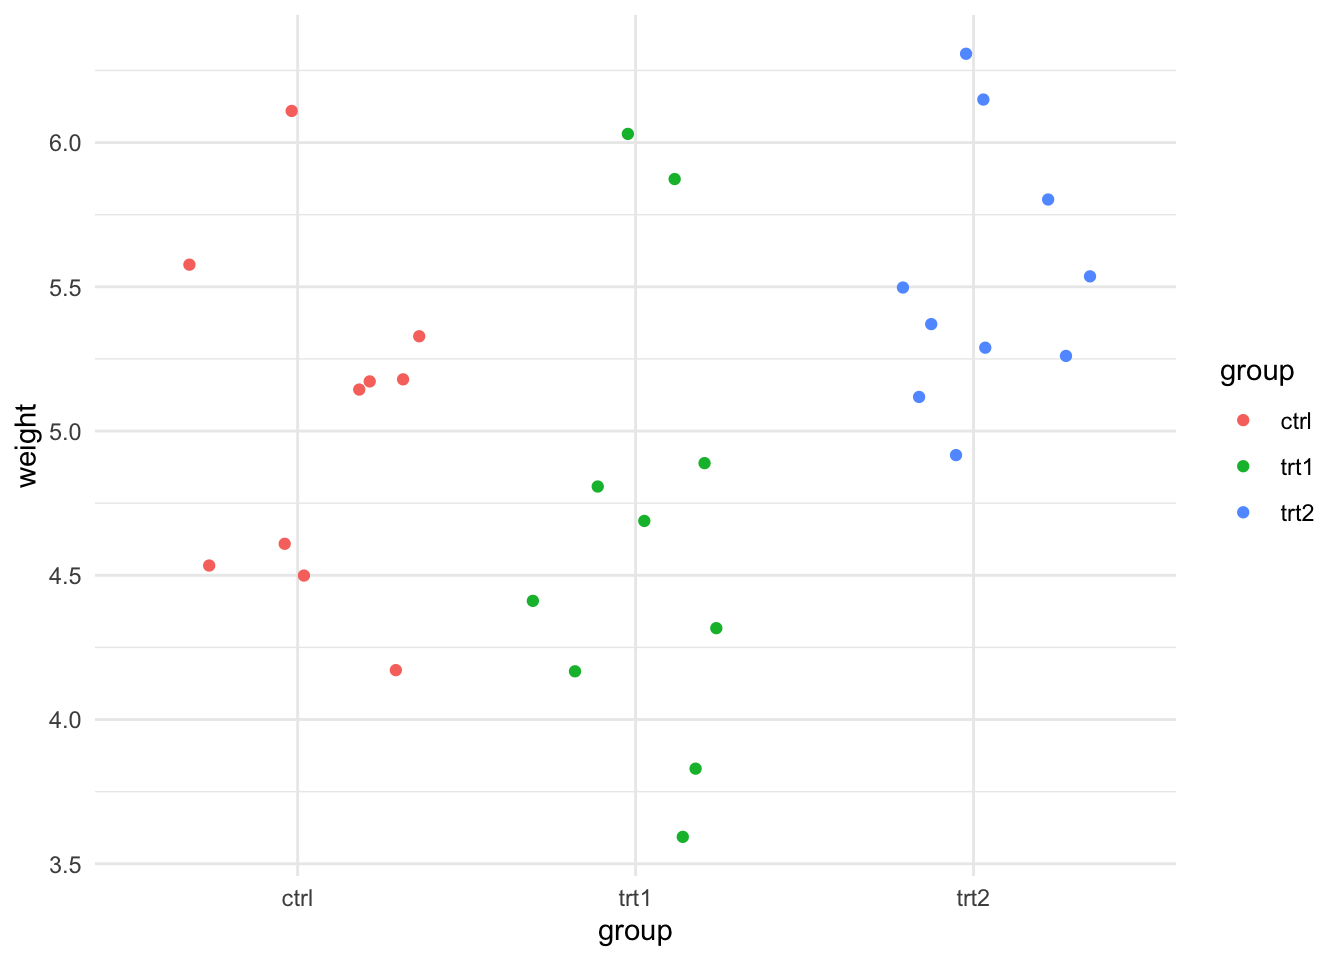
\includegraphics{bayes_factors_files/figure-latex/unnamed-chunk-21-1.pdf}

We will use this as an example data set, specifically we'll use \texttt{ctrl} and \texttt{trt2} data, which we need to extract. Note the mean values for \texttt{trt2} look larger than \texttt{ctrl}.

\begin{Shaded}
\begin{Highlighting}[]
\KeywordTok{library}\NormalTok{(dplyr)}
\NormalTok{pg_small <-}\StringTok{ }\NormalTok{PlantGrowth }\OperatorTok\StringTok{ }
\StringTok{  }\KeywordTok{filter}\NormalTok{(group }\OperatorTok\StringTok{ }\KeywordTok{c}\NormalTok{(}\StringTok{"trt2"}\NormalTok{, }\StringTok{"ctrl"}\NormalTok{)) }\OperatorTok\StringTok{ }
\StringTok{  }\KeywordTok{droplevels}\NormalTok{()}
\end{Highlighting}
\end{Shaded}

let's calculate too the sample difference mean and the standardised effect size, as it will be important to know these values later

\begin{Shaded}
\begin{Highlighting}[]
\KeywordTok{library}\NormalTok{(tidyr)}
\NormalTok{pg_small }\OperatorTok\StringTok{ }
\StringTok{  }\KeywordTok{group_by}\NormalTok{(group) }\OperatorTok\StringTok{ }
\StringTok{  }\KeywordTok{summarise}\NormalTok{(}\DataTypeTok{mean_weight =} \KeywordTok{mean}\NormalTok{(weight)) }\OperatorTok\StringTok{ }
\StringTok{  }\KeywordTok{pivot_wider}\NormalTok{( }\DataTypeTok{names_from =}\NormalTok{ group, }\DataTypeTok{values_from =}\NormalTok{ mean_weight) }\OperatorTok\StringTok{ }
\StringTok{  }\KeywordTok{summarise}\NormalTok{(}\DataTypeTok{mean_sample_diff =} \StringTok{`}\DataTypeTok{trt2}\StringTok{`} \OperatorTok{-}\StringTok{ `}\DataTypeTok{ctrl}\StringTok{`}\NormalTok{)}
\end{Highlighting}
\end{Shaded}

\begin{verbatim}
## # A tibble: 1 x 1
##   mean_sample_diff
##              <dbl>
## 1            0.494
\end{verbatim}

So the mean of \texttt{trt2} is bigger than \texttt{ctrl} by 0.49 g.

\begin{Shaded}
\begin{Highlighting}[]
\KeywordTok{library}\NormalTok{(effectsize)}
\KeywordTok{cohens_d}\NormalTok{(weight }\OperatorTok{~}\StringTok{ }\NormalTok{group, }\DataTypeTok{data=}\NormalTok{pg_small)}
\end{Highlighting}
\end{Shaded}

\begin{verbatim}
## Cohen's d |         95% CI
## --------------------------
## -0.95     | [-1.87, -0.01]
## 
## - Estimated using pooled SD.
\end{verbatim}

And correspondingly the standardised effect size is large. The effect size is negative because the calculation has been done in the order that the groups appear in the data. \texttt{ctrl} comes first so the calculation was \texttt{ctrl} - \texttt{trt2} which is a negative value. For now, this won't matter. We will need to pay attention to it later.

\hypertarget{two-sample-t-test}{%
\subsection{\texorpdfstring{Two Sample \(t\)-test}{Two Sample t-test}}\label{two-sample-t-test}}

Let's now do the \(t\)-tests. The hypotheses for a test comparing the treatment groups are

\begin{itemize}
\tightlist
\item
  \(H_0 : \bar{trt2} - \bar{ctrl} = 0\) IE the mean sample difference is 0
\item
  \(H_1 : \bar{trt2} - \bar{ctrl} \neq 0\) IE the mean sample difference is not 0
\end{itemize}

Using these data to do a \(t\)-test is easy, we'll specify a cut-off of 0.05 for rejection of \(H_0\).

\begin{Shaded}
\begin{Highlighting}[]
\NormalTok{model <-}\StringTok{ }\KeywordTok{lm}\NormalTok{(weight }\OperatorTok{~}\StringTok{ }\NormalTok{group, }\DataTypeTok{data =}\NormalTok{ pg_small)}
\KeywordTok{summary}\NormalTok{(model)}
\end{Highlighting}
\end{Shaded}

\begin{verbatim}
## 
## Call:
## lm(formula = weight ~ group, data = pg_small)
## 
## Residuals:
##    Min     1Q Median     3Q    Max 
## -0.862 -0.410 -0.006  0.280  1.078 
## 
## Coefficients:
##             Estimate Std. Error t value Pr(>|t|)    
## (Intercept)   5.0320     0.1637  30.742   <2e-16 ***
## grouptrt2     0.4940     0.2315   2.134   0.0469 *  
## ---
## Signif. codes:  0 '***' 0.001 '**' 0.01 '*' 0.05 '.' 0.1 ' ' 1
## 
## Residual standard error: 0.5176 on 18 degrees of freedom
## Multiple R-squared:  0.2019, Adjusted R-squared:  0.1576 
## F-statistic: 4.554 on 1 and 18 DF,  p-value: 0.04685
\end{verbatim}

We get a \(p\)-value of 0.046 which is less than our cut-off of 0.05 so we reject \(H_0\) as unlikely and accept \(H_1\) without explicitly testing it. Our conclusion scientifically is that \texttt{trt2} has greater \texttt{weight} than \texttt{ctrl}.

\hypertarget{a-bayesian-t-test}{%
\section{\texorpdfstring{A Bayesian \(t\)-test}{A Bayesian t-test}}\label{a-bayesian-t-test}}

Now let's set up a BayesFactor \(t\)-test. First we must set our hypotheses. The null hypothesis is similar to that in the frequentist \(t\)-test, the idea is that there is no effect which we formulated above as

\begin{itemize}
\tightlist
\item
  \(H_0 : \bar{trt2} - \bar{ctrl} = 0\) IE the mean sample difference is 0
\end{itemize}

Another way to say this is that the effect size \(d\) is 0 so

\begin{itemize}
\tightlist
\item
  \(H_0 : d = 0\)
\end{itemize}

Because we need something to compare against we now need to form the alternative hypothesis. By default the \texttt{ttestBF()} function tests the alternative hypothesis that the effect size is not 0

\begin{itemize}
\tightlist
\item
  \(H_1 : d \neq 0\)
\end{itemize}

and returns the Bayes Factor we need. Performing the test is straightforward

\begin{Shaded}
\begin{Highlighting}[]
\KeywordTok{library}\NormalTok{(BayesFactor)}
\KeywordTok{ttestBF}\NormalTok{(}\DataTypeTok{formula =}\NormalTok{  weight }\OperatorTok{~}\StringTok{ }\NormalTok{group, }\DataTypeTok{data =}\NormalTok{ pg_small)}
\end{Highlighting}
\end{Shaded}

\begin{verbatim}
## Bayes factor analysis
## --------------
## [1] Alt., r=0.707 : 1.774688 ±0%
## 
## Against denominator:
##   Null, mu1-mu2 = 0 
## ---
## Bayes factor type: BFindepSample, JZS
\end{verbatim}

We get a clear answer, the output on the line marked\texttt{{[}1{]}} is a Bayes Factor and states that the data are 1.77 times more likely if \(H_1\) were true than if \(H_0\) were true. In other words the odds of the data favouring the \(H_1\) to \(H_0\) are 1.77:1. Which is the answer we wanted to get, we have explicitly tested \(H_0\) and \(H_1\) and found that \(H_1\) is more likely to fit the data.

\hypertarget{comparing-p-and-the-bayes-factor-for-the-plantgrowth-data}{%
\section{\texorpdfstring{Comparing \(p\) and the Bayes Factor for the PlantGrowth data}{Comparing p and the Bayes Factor for the PlantGrowth data}}\label{comparing-p-and-the-bayes-factor-for-the-plantgrowth-data}}

Comparing to our table of interpretation of Bayes Factors, we see that this corresponds only to `Anecdotal Evidence' in favour of \(H_1\). Do we find this surprising given that the \(p\)-value from the \(t\)-test was significant? Does this mean that the two methods disagree? Strictly speaking, no, we shouldn't be surprised and no they don't disagree.

It's a bit of an apples and oranges situation. The two values are answers to very different questions.

As we've said before the frequentist \(p\)-value only measures the proportion of times a difference of the measured size would occur under some presumed background model. It does not measure the evidence that the hypothesis is true even though that is how many people try to interpret it. \(p\) only tells us how often we would be wrong if we reject \(H_0\). As a result many philosophers have stated that \(p\) based significance is a fundamentally uninteresting measure - who cares how often a difference occurs in some ideal world - what is important is the relative fit of the competing hypotheses to the data and that this measure of the strength of evidence per hypothesis is more in line with the interests of researchers.

Taken together our \(p\)-value states that the difference between the means of \texttt{trt2} and \texttt{ctrl} we observed occurs by chance in a normal distribution less than 0.05\% of the time and the Bayes Factor tells us that the odds that the data favour the idea that \texttt{trt2} is not the same as \texttt{ctrl} are only 1.7 times greater than the idea that \texttt{trt2} and \texttt{ctrl} are equal. We can see that the two methods do not contradict.

Hopefully this brings home the idea that Bayes Factor is different and arguably closer to what many scientists think they are doing when they do frequentist statistics.

Interpreting these results correctly, then, logically means that a researcher is not likely to be very excited by the results and would not over value the significance of the observed difference.

\hypertarget{better-hypotheses---one-tailed-tests}{%
\section{Better Hypotheses - One-tailed tests}\label{better-hypotheses---one-tailed-tests}}

But looking at the hypotheses we generated, could we ask a better, more informative one? With frequentist tests, no, but with Bayes Factors we can test different hypothesis. Instead of asking whether \texttt{trt2} is the same as \texttt{ctrl} or not we could ask something more specific. We are likely interested in whether \texttt{trt2} is greater than \texttt{ctrl}, or in other words that the effect size is greater than 0

\begin{itemize}
\tightlist
\item
  \(H_1 : d > 0\)
\end{itemize}

We can specify this \(H_1\) by setting the \texttt{nullInterval} argument, this is just the range we expect the effect sizes to be in under the null hypothesis, so we can use 0 to Infinity to cover any increased effect size (and -Infinity to 0 for any decreased effect size.

\hypertarget{a-data-frame-based-gotcha}{%
\subsection{A data frame based gotcha}\label{a-data-frame-based-gotcha}}

Here is where we can run afoul of R's idiosyncarcies - it is important to be careful here because the order of the data in the dataframe can have an effect that can confuse us. Recall that our effect size calculation for these data came out negative because \texttt{ctrl} came before \texttt{trt2}. Look at the dataframe \texttt{pg\_small}.

\begin{Shaded}
\begin{Highlighting}[]
\KeywordTok{str}\NormalTok{(pg_small)}
\end{Highlighting}
\end{Shaded}

\begin{verbatim}
## 'data.frame':    20 obs. of  2 variables:
##  $ weight: num  4.17 5.58 5.18 6.11 4.5 4.61 5.17 4.53 5.33 5.14 ...
##  $ group : Factor w/ 2 levels "ctrl","trt2": 1 1 1 1 1 1 1 1 1 1 ...
\end{verbatim}

Note that the \texttt{ctrl} level in the \texttt{group} factor is first, we need to think of our \(H_1\) more carefully,

\begin{itemize}
\tightlist
\item
  \(H_1 : d > 0\)
\end{itemize}

really is in this case

\begin{itemize}
\tightlist
\item
  \(H_1 : \bar{\text{trt2}} - \bar{\text{ctrl}} > 0\)
\end{itemize}

so we need to make sure that \texttt{trt2} comes first in the \texttt{group} factor. We can use the \texttt{\$} notation to reorder the factor as we wish

\begin{Shaded}
\begin{Highlighting}[]
\NormalTok{pg_small}\OperatorTok{$}\NormalTok{group <-}\StringTok{ }\KeywordTok{factor}\NormalTok{(pg_small}\OperatorTok{$}\NormalTok{group, }
                         \DataTypeTok{levels=}\KeywordTok{c}\NormalTok{(}\StringTok{"trt2"}\NormalTok{, }\StringTok{"ctrl"}\NormalTok{) )}
\KeywordTok{str}\NormalTok{(pg_small)}
\end{Highlighting}
\end{Shaded}

\begin{verbatim}
## 'data.frame':    20 obs. of  2 variables:
##  $ weight: num  4.17 5.58 5.18 6.11 4.5 4.61 5.17 4.53 5.33 5.14 ...
##  $ group : Factor w/ 2 levels "trt2","ctrl": 2 2 2 2 2 2 2 2 2 2 ...
\end{verbatim}

\hypertarget{performing-the-one-tailed-test}{%
\section{Performing the One-tailed test}\label{performing-the-one-tailed-test}}

With that done we can move back on with the one-sided test, specifying the interval as expected.

\begin{Shaded}
\begin{Highlighting}[]
\KeywordTok{ttestBF}\NormalTok{(}\DataTypeTok{formula =}\NormalTok{  weight }\OperatorTok{~}\StringTok{ }\NormalTok{group, }\DataTypeTok{data =}\NormalTok{ pg_small, }\DataTypeTok{nullInterval=}\KeywordTok{c}\NormalTok{(}\DecValTok{0}\NormalTok{, }\OtherTok{Inf}\NormalTok{))}
\end{Highlighting}
\end{Shaded}

\begin{verbatim}
## Bayes factor analysis
## --------------
## [1] Alt., r=0.707 0<d<Inf    : 3.387166  ±0%
## [2] Alt., r=0.707 !(0<d<Inf) : 0.1622109 ±0%
## 
## Against denominator:
##   Null, mu1-mu2 = 0 
## ---
## Bayes factor type: BFindepSample, JZS
\end{verbatim}

Performing the test was nice and easy and we get an answer. The first line of the output \texttt{{[}1{]}} states the odds that the data favour the alternative hypothesis over the null are 3.38:1. The Bayes Factor is increased over the earlier more vague hypothesis, suggesting there is actually substantial evidence for the idea that the effect size is greater than 0.

\hypertarget{testing-the-effect-of-the-prior}{%
\section{Testing the effect of the prior}\label{testing-the-effect-of-the-prior}}

We discussed that one of the limitations of Bayesian Inference was the need to carefully and justifiably select a prior and that doing so was difficult. We'll look at that a little bit now as we did make a decision on this albeit implicitly by allowing the defaults of the \texttt{ttestBF()} function.

In our \texttt{ttestBF()} function we actually need to provide a prior distribution for the maths to work, not just a single value. We don't want to get into details of those maths as they are out of scope but we do need to know that the prior distribution needs to cover a range of effect sizes that might be plausible if the null hypothesis were false.

The \texttt{BayesFactor} package provides a Cauchy distribution as default. Since the selection of the prior implies that we know something about our dat, using the Cauchy implies that we think the population is normally distributed (which is the same distribution we assume under the standard frequentist statistical tests).

\hypertarget{the-cauchy-prior-distribution}{%
\subsection{The Cauchy Prior Distribution}\label{the-cauchy-prior-distribution}}

The Cauchy is a distribution with a single parameter called \texttt{scale} that affects how wide its main humpy bit is. In \texttt{BayesFactor} there are three widths we can choose from depending on how big a difference we think we are seeing, that is how big the effect size. When plotted, these distributions look like this

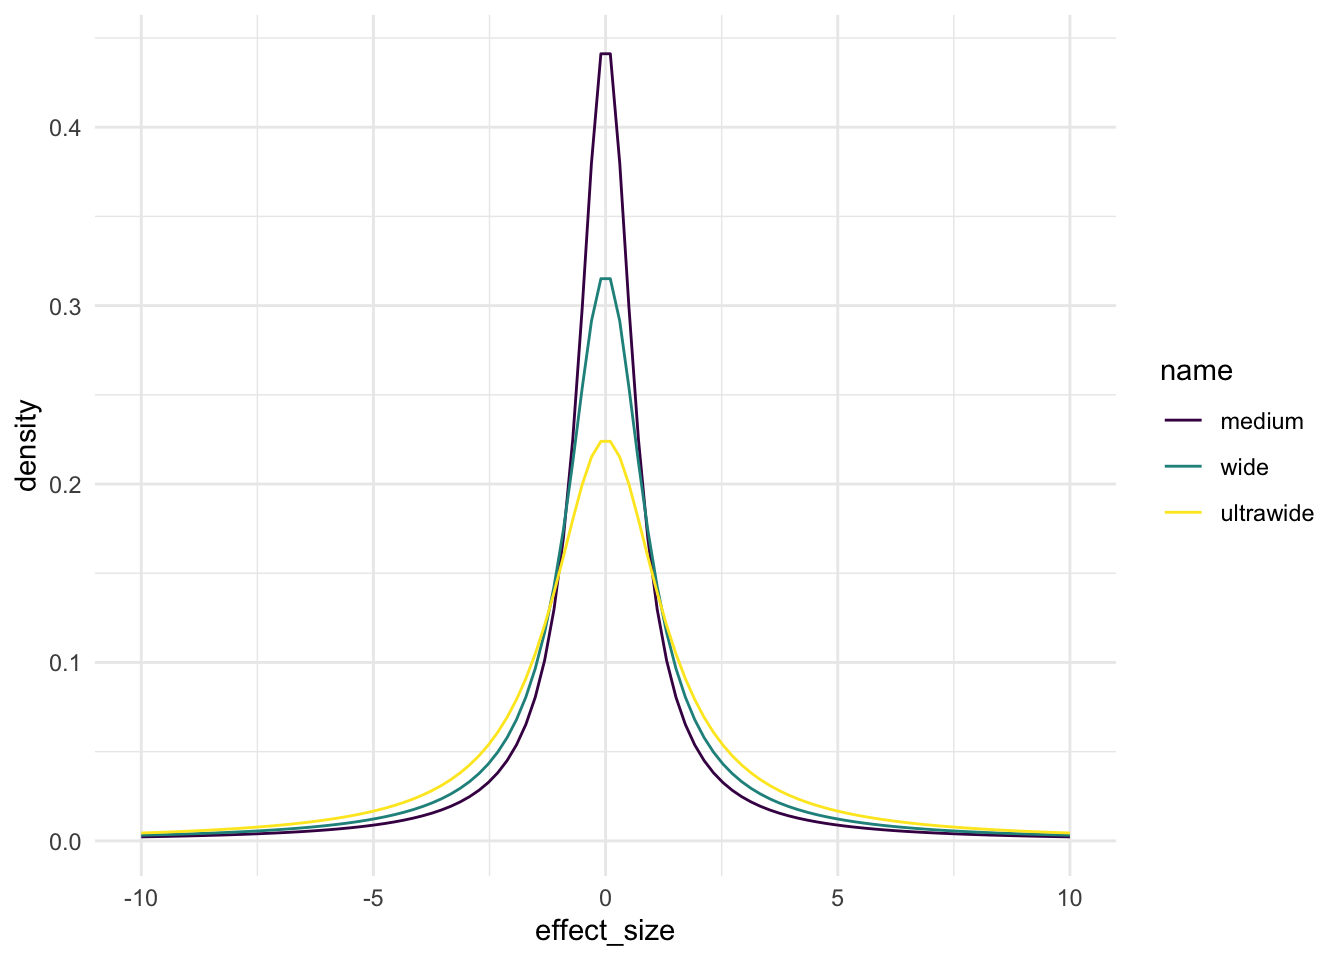
\includegraphics{bayes_factors_files/figure-latex/unnamed-chunk-30-1.pdf}

and the \texttt{name} corresponds to \texttt{scale} values as follows

\begin{tabular}{l|r}
\hline
name & scale\\
\hline
medium & 0.71\\
\hline
wide & 1.00\\
\hline
ultrawide & 1.41\\
\hline
\end{tabular}

In each of the distributions 50\% of the area under the curve falls within +/- the scale value.

Since the scale on the \(x\)-axis in our plot is effect size, the choice of scale values says somerthing about what we are expecting our effect sizes to be like. The wider the scale value, the bigger we are expecting our effect sizes to be.

Our effect size in the \texttt{PlantGrowth} data was 0.95 so well within the area covered by the \texttt{medium} scale Cauchy, much more of that curve falls within the -0.95 to +0.95 effect size range than the other two, so we might think that one would be a better fit. That's why it's the default, it's a good fit for generally found effect sizes.

\hypertarget{the-effect-of-changing-the-prior}{%
\subsection{The effect of changing the prior}\label{the-effect-of-changing-the-prior}}

As an exercise to help us understand the importance of the prior and explicitly NOT a guide to maximising the odds in favour of one model over another. Let's look at how changing the scale via the \texttt{rscale} parameter in \texttt{ttestBF()} affects the odds of our one sided model.

\begin{Shaded}
\begin{Highlighting}[]
\KeywordTok{ttestBF}\NormalTok{(}\DataTypeTok{formula =}\NormalTok{  weight }\OperatorTok{~}\StringTok{ }\NormalTok{group, }\DataTypeTok{data =}\NormalTok{ pg_small, }\DataTypeTok{nullInterval=}\KeywordTok{c}\NormalTok{(}\DecValTok{0}\NormalTok{, }\OtherTok{Inf}\NormalTok{), }\DataTypeTok{rscale=}\StringTok{"medium"}\NormalTok{)}
\end{Highlighting}
\end{Shaded}

\begin{verbatim}
## Bayes factor analysis
## --------------
## [1] Alt., r=0.707 0<d<Inf    : 3.387166  ±0%
## [2] Alt., r=0.707 !(0<d<Inf) : 0.1622109 ±0%
## 
## Against denominator:
##   Null, mu1-mu2 = 0 
## ---
## Bayes factor type: BFindepSample, JZS
\end{verbatim}

\begin{Shaded}
\begin{Highlighting}[]
\KeywordTok{ttestBF}\NormalTok{(}\DataTypeTok{formula =}\NormalTok{  weight }\OperatorTok{~}\StringTok{ }\NormalTok{group, }\DataTypeTok{data =}\NormalTok{ pg_small, }\DataTypeTok{nullInterval=}\KeywordTok{c}\NormalTok{(}\DecValTok{0}\NormalTok{, }\OtherTok{Inf}\NormalTok{), }\DataTypeTok{rscale=}\StringTok{"wide"}\NormalTok{)}
\end{Highlighting}
\end{Shaded}

\begin{verbatim}
## Bayes factor analysis
## --------------
## [1] Alt., r=1 0<d<Inf    : 3.22134   ±0%
## [2] Alt., r=1 !(0<d<Inf) : 0.1189759 ±0%
## 
## Against denominator:
##   Null, mu1-mu2 = 0 
## ---
## Bayes factor type: BFindepSample, JZS
\end{verbatim}

\begin{Shaded}
\begin{Highlighting}[]
\KeywordTok{ttestBF}\NormalTok{(}\DataTypeTok{formula =}\NormalTok{  weight }\OperatorTok{~}\StringTok{ }\NormalTok{group, }\DataTypeTok{data =}\NormalTok{ pg_small, }\DataTypeTok{nullInterval=}\KeywordTok{c}\NormalTok{(}\DecValTok{0}\NormalTok{, }\OtherTok{Inf}\NormalTok{), }\DataTypeTok{rscale=}\StringTok{"ultrawide"}\NormalTok{)}
\end{Highlighting}
\end{Shaded}

\begin{verbatim}
## Bayes factor analysis
## --------------
## [1] Alt., r=1.414 0<d<Inf    : 2.857414   ±0%
## [2] Alt., r=1.414 !(0<d<Inf) : 0.08596477 ±0%
## 
## Against denominator:
##   Null, mu1-mu2 = 0 
## ---
## Bayes factor type: BFindepSample, JZS
\end{verbatim}

Indeed we do get stronger odds for the alternative hypothesis in the \texttt{medium} scale than the others. Note that it isn't wise to go Bayes Factor fishing by post-hoc selecting the prior in order to maximise the Bayes Factor. This example was an exercise to show that prior selection is important.

\begin{roundup}
\begin{itemize}
\tightlist
\item
  Bayes Factor \(t\)-tests allow us to directly compare hypothesis about data in a way that is analogous to \(t\)-tests.
\item
  We can compare different hypotheses
\item
  The interpretation of a BayesFactor tells us which of the hypotheses are favoured by the data
\item
  Prior selection is important, but \texttt{ttestBF()} restricts us to sensible options for data we assume to be normal
\end{itemize}
\end{roundup}

\hypertarget{bayes-factor-anova}{%
\chapter{Bayes Factor ANOVA}\label{bayes-factor-anova}}

\hypertarget{the-issue-of-multiplicity-in-frequentism-and-bayesianism}{%
\section{The issue of multiplicity in Frequentism and Bayesianism}\label{the-issue-of-multiplicity-in-frequentism-and-bayesianism}}

The ANOVA is often seen to be a catch-all test that can be used for an experiment that has more than two samples in it. Experimenters often understand this to be true on the basis that `you shouldn't do \(t\)-tests for more than two samples by repeating the \(t\)-test'. This is quite true and is a strategy for avoidance of the problem of multiplicity.

Multiplicity or multiple testing occurs when we do lots of tests one after the other, in a batch. The more we do, the more likely we are to make an error in our conclusions (not in our working). This happens in Frequentist statistical tests because the \(p\)-value expresses a fixed error rate that we are happy to accept.

Recall that the \(t\)-test evaluates two hypotheses

\(H_0 : \bar{x_1} - \bar{x_2} = 0\)

\(H_1 : \bar{x_1} - \bar{x_2} \neq 0\)

and we set a level at which would reject \(H_0\) usually \(p < 0.05\). The \(p\) reflects the proportion of times that the difference observed is seen in the null model by chance (so we see the difference 1 in 20 times by chance), in other words in a proportion of 0.95 of times we would reject the null correctly. Which is fine for just one comparison.

If we do more than one test we must multiply these probabilities together, giving \(0.95 * 0.95 = 0.9025\). This is catastrophic, by doing just two tests we reduce the proportion of times we choose the correct hypothesis to 0.9025, down from 19/20 to 18/20, we make twice as many mistakes! For more tests this gets worse.

Frequentist statistics have lots of corrections for this sort of problem and the ANOVA post-hoc tests are in part a way of doing that. The good news for those using Bayes Factors is that this problem does not exist. Because we don't have a fixed error rate, it doesn't get bigger when we do more tests. We are free to do as many hypothesis comparisons as we wish.

\hypertarget{automating-bayesfactorttest-for-many-comparisions}{%
\section{\texorpdfstring{Automating \texttt{BayesFactor::ttest()} for many comparisions}{Automating BayesFactor::ttest() for many comparisions}}\label{automating-bayesfactorttest-for-many-comparisions}}

As there isn't a need for a Bayes Factor analogue to the ANOVA and post-hoc tests, we can just use the \(t\)-test analogue over and over again. If we have a multiple sample dataset we just need a book-keeping method to pull out the samples of interest.

Let's draft one with \texttt{dplyr} and the Plant Growth data set.

\begin{Shaded}
\begin{Highlighting}[]
\KeywordTok{library}\NormalTok{(dplyr)}
\KeywordTok{library}\NormalTok{(BayesFactor)}

\NormalTok{small_df <-}\StringTok{ }\NormalTok{PlantGrowth }\OperatorTok\StringTok{ }
\StringTok{    }\KeywordTok{filter}\NormalTok{(group }\OperatorTok\StringTok{ }\KeywordTok{c}\NormalTok{(}\StringTok{"ctrl"}\NormalTok{, }\StringTok{"trt1"}\NormalTok{)) }\OperatorTok\StringTok{ }
\StringTok{    }\KeywordTok{droplevels}\NormalTok{()}
  
\KeywordTok{ttestBF}\NormalTok{(}\DataTypeTok{formula =}\NormalTok{ weight }\OperatorTok{~}\StringTok{ }\NormalTok{group, }\DataTypeTok{data =}\NormalTok{ small_df)}
\end{Highlighting}
\end{Shaded}

This pattern helps you extract the pairs of samples you need, though you would need to repeat it every time you wanted to analyse a new pair. A convenience function for the simple case that allows us to do \texttt{BayesFactor::ttestBF()} for all pairs in a specified column in a dataframe exists in the package \texttt{simplebf}. It works like this:

\begin{Shaded}
\begin{Highlighting}[]
\KeywordTok{library}\NormalTok{(simplebf)}
\NormalTok{result <-}\StringTok{ }\KeywordTok{allpairs_ttestbf}\NormalTok{(PlantGrowth, }
                           \DataTypeTok{group_col =} \StringTok{"group"}\NormalTok{, }\DataTypeTok{data_col =} \StringTok{"weight"}\NormalTok{, }
                           \DataTypeTok{rscale =} \StringTok{"medium"}\NormalTok{, }
                           \DataTypeTok{h_1 =} \StringTok{"test_greater_than_control"}\NormalTok{)}

\NormalTok{knitr}\OperatorTok{::}\KeywordTok{kable}\NormalTok{(result, }\DataTypeTok{digits =} \DecValTok{4}\NormalTok{)}
\end{Highlighting}
\end{Shaded}

\begin{tabular}{l|l|l|l|r|l|l}
\hline
control\_group & test\_group & h\_0 & h\_1 & BayesFactor & odds\_h\_1 & summary\\
\hline
trt1 & ctrl & ctrl equal to trt1 & ctrl greater than trt1 & 1.0834 & 1:1.0834 & Anecdotal evidence for H\_1 compared to H\_0\\
\hline
trt2 & ctrl & ctrl equal to trt2 & ctrl greater than trt2 & 0.1622 & 1:0.1622 & Substantial evidence for H\_0 compared to H\_1\\
\hline
ctrl & trt1 & trt1 equal to ctrl & trt1 greater than ctrl & 0.2167 & 1:0.2167 & Substantial evidence for H\_0 compared to H\_1\\
\hline
trt2 & trt1 & trt1 equal to trt2 & trt1 greater than trt2 & 0.1363 & 1:0.1363 & Substantial evidence for H\_0 compared to H\_1\\
\hline
ctrl & trt2 & trt2 equal to ctrl & trt2 greater than ctrl & 3.3872 & 1:3.3872 & Substantial evidence for H\_1 compared to H\_0\\
\hline
trt1 & trt2 & trt2 equal to trt1 & trt2 greater than trt1 & 12.6445 & 1:12.6445 & Strong evidence for H\_1 compared to H\_0\\
\hline
\end{tabular}

The results are pretty easy to read. Note we can set \texttt{rscale} values as in the \texttt{ttestBF()} and we can choose one of three values for \(H_1\) \texttt{test\_greater\_than\_control}, \texttt{test\_less\_than\_control} and \texttt{test\_not\_equal\_to\_control}.

\begin{roundup}
\begin{itemize}
\tightlist
\item
  Bayes Factors do not need multiple hypothesis corrections
\item
  \texttt{simplebf} is a package for automating the comparison of all groups in a single variable in a tidy dataframe
\end{itemize}
\end{roundup}

\hypertarget{bayes-factor-chi2}{%
\chapter{\texorpdfstring{Bayes Factor \(\chi^2\)}{Bayes Factor \textbackslash chi\^{}2}}\label{bayes-factor-chi2}}

  \bibliography{book.bib,packages.bib}

\end{document}
